\section{The pipeline}

\gourd\ has a strict pipeline built on a custom docker container.

\begin{center}
  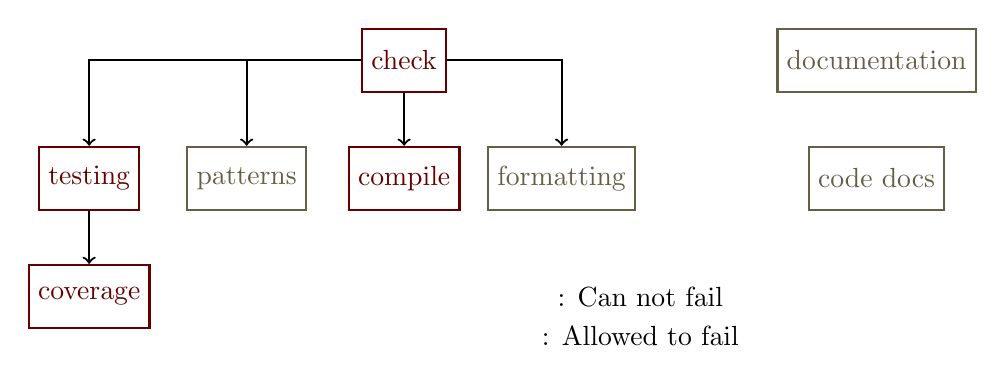
\begin{tikzpicture}
    \node (check) at (0,0) [draw,thick,minimum width=1cm,minimum height=0.8cm,color=red!40!black] {check};
    \node (build) [draw,thick,minimum width=1cm,minimum height=0.8cm,color=red!40!black, below of=check, yshift=-0.5cm] {compile};
    \node (fmt) [draw,thick,minimum width=1cm,minimum height=0.8cm,color=yellow!30!black, below of=check, yshift=-0.5cm, xshift=2cm] {formatting};
    \node (test) [draw,thick,minimum width=1cm,minimum height=0.8cm,color=red!40!black, below of=check, yshift=-0.5cm, xshift=-4cm] {testing};
    \node (cov) [draw,thick,minimum width=1cm,minimum height=0.8cm,color=red!40!black, below of=test, yshift=-0.5cm] {coverage};
    \node (clippy) [draw,thick,minimum width=1cm,minimum height=0.8cm,color=yellow!30!black, below of=check, yshift=-0.5cm, xshift=-2cm] {patterns};


    \node (doc) at (6,0) [draw,thick,minimum width=1cm,minimum height=0.8cm,color=yellow!30!black] {documentation};
    \node (rdoc) [draw,thick,minimum width=1cm,minimum height=0.8cm,color=yellow!30!black, below of=doc, yshift=-0.5cm] {code docs};

    \draw[thick, ->] (check) -- (build);
    \draw[thick, ->] (check) -| (fmt);
    \draw[thick, ->] (check) -| (clippy);
    \draw[thick, ->] (check) -| (test);
    \draw[thick, ->] (test) -- (cov);

    \node at (3, -3) {\textcolor{red!40!black}{$\blacksquare$}: Can not fail};
    \node at (3, -3.5) {\textcolor{yellow!30!black}{$\blacksquare$}: Allowed to fail};
  \end{tikzpicture}
  \captionof{figure}{An overview of the pipeline}
\end{center}

The pipeline configuration is fully contained in \texttt{.gitlab-ci.yml} in the
root of the project.

Currently the docker container is hosted in a public GitHub repository, because
there was a need to publish it in a container registry if there is a need for
updating Rust or migration of the pipeline this container will have to be
rebuilt.

There are three containers that are needed for the pipeline:

\begin{enumerate}
  \item A container with Rust stable, MSRV version.
  \item A container with Rust nightly, \texttt{rustfmt}, \texttt{clippy}.
  \item A container with all of TexLive and Rust, MSRV or nightly.
\end{enumerate}

These three are defined at the top of the file and if the pipeline is ever updated
or migrated these should be updated. All three containers are built on top of
musl systems for minimal footprint. (In fact the GitHub container is based off of \texttt{musl-rust})
